\documentclass[runningheads]{llncs}

% ---------------------------------------------------------------
% ECCV/LNCS review template
\usepackage[review,year=2026,ID=*****]{eccv}
% \usepackage{eccv}

\usepackage{eccvabbrv}
\usepackage{graphicx}
\usepackage{booktabs}
\usepackage{float}
\usepackage{amsmath}   % [EDIT] align/cases; harmless if eccv.sty already loads it
\usepackage{amssymb}   % [EDIT] \mathbb{R}
\usepackage[accsupp]{axessibility}
\usepackage[pagebackref,breaklinks,colorlinks,citecolor=eccvblue]{hyperref}
\usepackage{orcidlink}

\begin{document}

\title{MarineMamba: Multi-Granularity CLIP Feature Integration with Dual Mamba for Underwater Classification}
\titlerunning{MarineMamba}

\author{Anonymous ECCV Submission}
\authorrunning{Anonymous}
\institute{Paper ID *****}

\maketitle

\begin{abstract}
Underwater species recognition supports marine monitoring, aquaculture, and coral-reef assessment, but remains difficult because classes are fine-grained, images are degraded by underwater optics, and naturally collected datasets are often long-tailed. We present MarineMamba, a lightweight classifier that keeps two CLIP visual encoders (ViT-B/16 and ViT-B/32) frozen and trains only a dual-branch state-space head. Each branch projects CLIP's spatial grid, prepends the corresponding CLIP feature vector, scans the spatial tokens in bidirectional spiral order, and refines the restored feature map with channel-and-spatial attention. The two branch descriptors are then fused for classification with a class-weighted focal loss. With 1.03M trainable parameters, MarineMamba reaches $93.46\pm0.57\%$ top-1 accuracy on AQUA20 and $95.90\pm0.80\%$ on Sea Animals 23, outperforming fVim-tiny, our fully fine-tuned Vim-tiny baseline, while training roughly $7\times$ fewer parameters. On the raw, 881:1-imbalanced Fish4Knowledge split, it reaches $98.25\pm0.26\%$, $1.50$ points behind the same baseline. Against a frozen-CLIP MLP that discards the spatial grid, MarineMamba adds $4.13$ points on AQUA20. Ablations indicate that the Mamba layer is most valuable for propagating the injected CLIP feature vector across spatial tokens before pooling, while spiral scanning mainly improves accuracy stability across random seeds.
\keywords{Underwater recognition \and CLIP \and Mamba \and State-space models}
\end{abstract}

\section{Introduction}
\label{sec:intro}

Automated recognition of aquatic and marine species is central to biodiversity surveys, fisheries stock assessment, aquaculture monitoring, and coral-reef health assessment~\cite{gonzalez2023underwater}. Manual annotation of underwater video and still imagery does not scale to modern camera-trap and autonomous-vehicle deployments, but underwater recognition is not a direct copy of natural-image classification. Species are often separated by subtle body-shape, fin, texture, or color-pattern differences; images suffer from wavelength-dependent color attenuation, scattering, blur, and non-uniform illumination; and field collections are naturally long-tailed. In the Fish4Knowledge~\cite{fish4knowledge} split used in this paper, the most frequent training class contains 9{,}690 images whereas the rarest contains only 11, yielding an 881:1 imbalance ratio.

These properties make full backbone fine-tuning a fragile default. Marine datasets are usually smaller and more imbalanced than the pretraining corpora used for modern CNN, Transformer, or state-space backbones~\cite{he2016resnet,dosovitskiy2021vit,gu2024mamba}, so updating all backbone weights can overfit to a particular deployment, split, or species list. A complementary strategy is to freeze a broadly pretrained visual encoder and learn only a small, domain-specific head. CLIP~\cite{radford2021clip} is well suited to this regime because its image encoder provides transferable global and spatial features, while CLIP ViT-B/16 and ViT-B/32 expose two granularities of evidence from the same image. The remaining question is how to use the spatial grids rather than only the pooled feature vectors.

State-space models provide a useful mechanism for this head because they propagate information through a linear-time recurrence. Mamba~\cite{gu2024mamba} and visual variants such as Vim~\cite{zhu2024vim}, VMamba~\cite{liu2024vmamba}, and LocalMamba~\cite{huang2024localmamba} have made selective state-space modeling a growing direction in vision~\cite{zhang2024visualmambasurvey}. These models also show that token ordering is not a minor implementation choice: a sequential model can only process a two-dimensional image grid after the grid has been serialized. Raster order creates artificial discontinuities at row boundaries, and those discontinuities are especially visible on the small CLIP feature grids used here. This motivates a spatial head that keeps the CLIP encoders frozen, preserves local adjacency during scanning, and fuses fine- and coarse-grained evidence without training a large backbone.

We propose MarineMamba, a dual-branch classifier for underwater and aquatic species recognition. The method extracts frozen CLIP ViT-B/16 and ViT-B/32 spatial grids and feature vectors, projects each granularity into a compact hidden space, prepends the corresponding CLIP feature vector to the spatial tokens, and processes the sequence with a bidirectional spiral-scan Mamba block. After restoring the spatial layout, channel-and-spatial attention refines each branch; the two descriptors are concatenated and classified. Because the CLIP encoders are never updated, MarineMamba trains only 1.03M parameters while still using both global CLIP evidence and spatial patch structure.

The main contributions are:
\begin{itemize}
  \item a lightweight frozen-CLIP recognition pipeline for underwater and aquatic species classification, using ViT-B/16 and ViT-B/32 grids as complementary granularities;
  \item a MarineMamba block that combines feature-vector injection, bidirectional spiral scanning, Mamba sequence modeling, and channel-and-spatial attention for small CLIP feature grids;
  \item experiments on AQUA20, Sea Animals 23, and Fish4Knowledge showing strong top-1 accuracy with substantially fewer trainable parameters than fVim-tiny, a fully fine-tuned Vim-tiny baseline;
  \item ablations that separate the contribution of spatial-grid modeling from the contribution of CLIP pretraining and identify both the benefits and limitations of the proposed head.
\end{itemize}

\section{Related Work}
\label{sec:related}

\textbf{Marine and Underwater Recognition.}
Marine image recognition, situated within the broader underwater computer vision landscape~\cite{gonzalez2023underwater}, has followed the movement from hand-crafted features to fully learned backbones. CNNs such as ResNet~\cite{he2016resnet}, EfficientNet~\cite{tan2019efficientnet}, and ConvNeXt~\cite{liu2022convnext} provide hierarchical local features, while Vision Transformers~\cite{dosovitskiy2021vit} replace convolutional aggregation with global self-attention. In underwater settings, these architectures must operate under color attenuation, scattering, background clutter, fine-grained species similarity, and uneven class frequencies. These factors make the evaluation protocol especially important: accuracy on a curated or balanced split may not reflect performance on naturally collected data.

Fish4Knowledge~\cite{fish4knowledge} is a representative benchmark for fish-species recognition. MLR-VGGNet~\cite{prasetyo2021resvggnet} reports $99.69\%$ accuracy under a curated, class-balanced split, while ConvFishNet~\cite{qu2024convfishnet}, inspired by FishNet~\cite{sun2018fishnet}, reports high precision on a natural split with substantially reduced computational cost. These methods demonstrate the effectiveness of specialized CNN designs for marine imagery, but their reported numbers are difficult to compare directly with raw long-tailed splits because preprocessing, partitions, and class distributions differ. More recent datasets and studies broaden this setting: AQUA20~\cite{fuad2026aqua20} provides a challenging aquatic species benchmark, and AquaSelect~\cite{daga2026aquaselect} studies selective prediction so a trained classifier can abstain when confidence is low. These works highlight complementary problems: stronger marine representations, reliable confidence, and robustness to imbalance.

\textbf{Mamba-Based Vision Methods.}
State-space models offer a different route to global context, and recent surveys identify visual recognition as a central application area for Mamba-style architectures~\cite{zhang2024visualmambasurvey}. S4~\cite{gu2022s4} and Mamba~\cite{gu2024mamba} model long sequences through linear-time recurrence rather than quadratic self-attention. Vision adaptations therefore need a rule for serializing image grids. Vim~\cite{zhu2024vim} applies bidirectional state-space modeling to visual tokens, VMamba~\cite{liu2024vmamba} aggregates multiple directional scans, LocalMamba~\cite{huang2024localmamba} emphasizes local windows, and PlainMamba~\cite{yang2024plainmamba} studies non-hierarchical visual Mamba models. Together, these works make scan order a core modeling choice rather than a preprocessing detail.

Several Mamba studies are especially relevant to spatial ordering and feature fusion. SpiralMamba~\cite{spiralmamba} and LSFMamba~\cite{lsfmamba} show that spiral traversal can be useful when local continuity matters, particularly in hyperspectral classification. Closest in spirit to CLIP-guided state-space modeling, M$^3$amba~\cite{cao2025m3amba} couples CLIP with a Mamba fusion module for multi-modal remote sensing, but it targets sensor fusion rather than marine RGB species recognition.

Existing marine-recognition methods mostly rely on fully fine-tuned CNN or Transformer backbones, often under dataset protocols that differ in split construction and imbalance severity. Existing visual Mamba methods, in turn, focus mainly on generic recognition, hyperspectral data, remote-sensing fusion, or modality-specific adaptation, and they do not directly address frozen multi-granularity CLIP feature grids for long-tailed underwater species classification. MarineMamba enters this gap by keeping the CLIP encoders frozen, using a small trainable state-space head, and scanning the fine and coarse CLIP spatial grids with locality-preserving spiral order before fusing them for classification.

\section{Methodology}
\label{sec:method}

MarineMamba separates visual representation learning from task-specific classification. Two frozen CLIP visual encoders provide complementary spatial features, and a compact state-space classifier --- the only trainable component --- models their fine- and coarse-scale structure. The fine branch operates on local patch evidence from CLIP ViT-B/16, the coarse branch on the broader context of CLIP ViT-B/32. Each branch injects the corresponding CLIP feature vector into a spiral-ordered Mamba sequence, and the two branch descriptors are concatenated before classification. \Cref{fig:architecture} gives an overview.

Throughout, $r\in\{16,32\}$ indexes the two granularities, $H_r\times W_r$ is the extent of the corresponding CLIP feature grid ($14\times14$ and $7\times7$), $N_r=H_rW_r$, $d=128$ is the shared hidden width, and $C$ is the number of species. We write $[\cdot\,;\cdot]$ for concatenation along the token dimension and $\odot$ for the Hadamard product.

\begin{figure}[t]
  \centering
  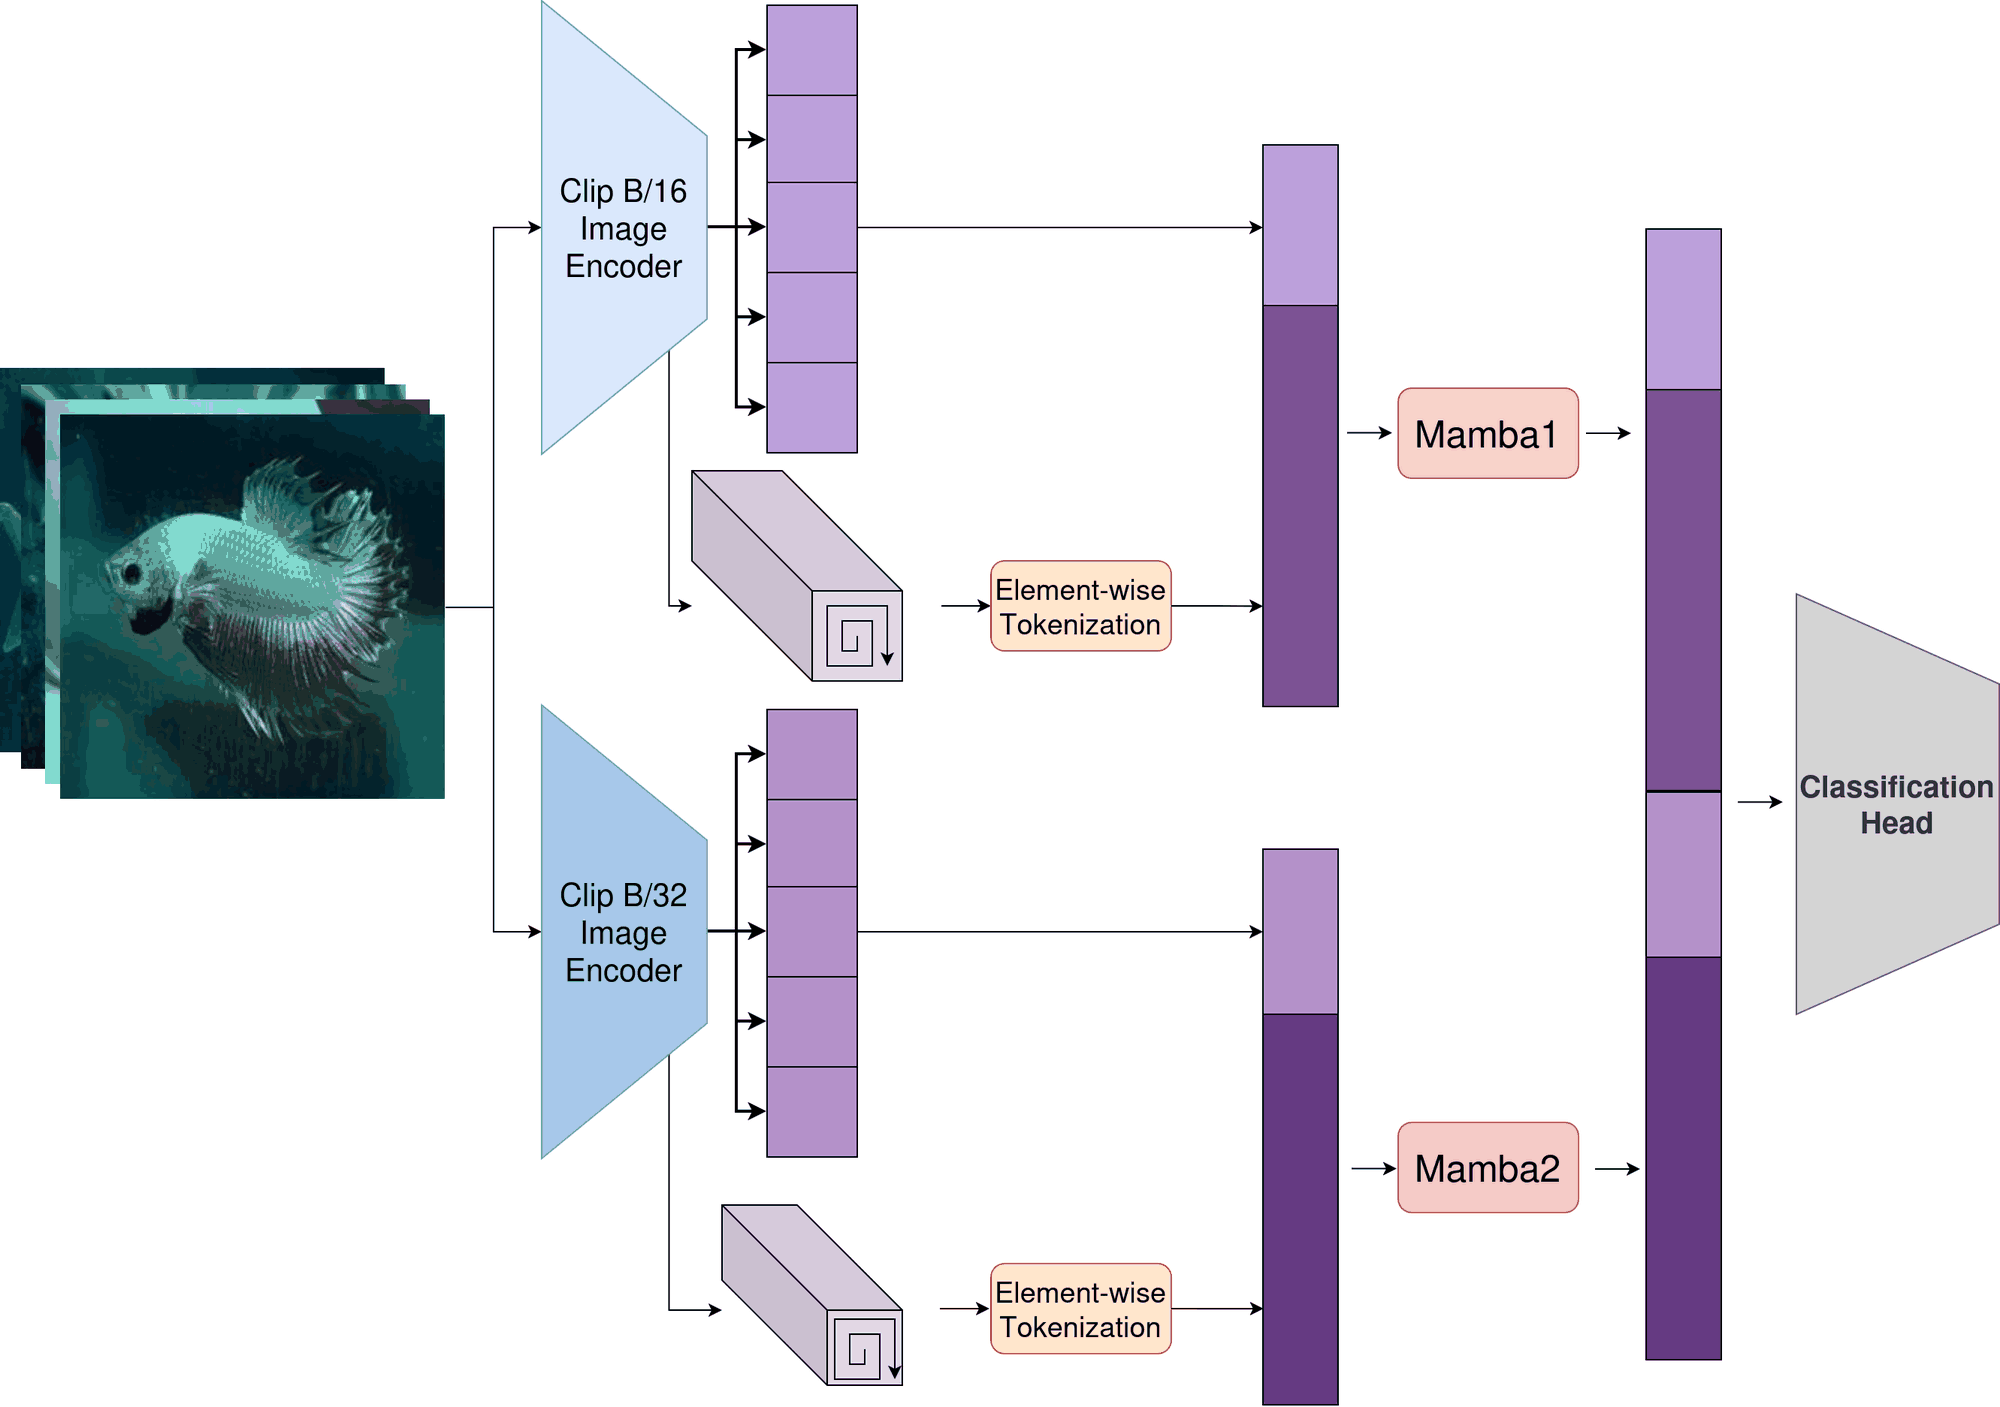
\includegraphics[width=0.78\linewidth]{figures/mamba.drawio.png}
  \caption{Overview of MarineMamba. Frozen CLIP ViT-B/16 and ViT-B/32 encoders provide fine and coarse feature grids plus global CLIP feature vectors. Each branch performs spiral-ordered Mamba modeling, and the two descriptors are concatenated for classification.}
  \label{fig:architecture}
\end{figure}

\subsection{Multi-Granularity CLIP Feature Extraction}
\label{sec:method-clip}

% [EDIT] The old Eq. (1) was a numbered equation that only said "call the encoder".
% Demoted to prose; the information content (shapes) is now stated explicitly.
Given an input image $x$, two frozen CLIP visual encoders $\Phi_{16}$ and $\Phi_{32}$ produce a spatial feature grid together with a global embedding, $(\mathbf{S}_r,\mathbf{g}_r)=\Phi_r(x)$, with
\begin{equation*}
  \mathbf{S}_r \in \mathbb{R}^{768\times H_r\times W_r},
  \qquad
  \mathbf{g}_r \in \mathbb{R}^{512},
  \qquad r\in\{16,32\}.
\end{equation*}
Neither encoder is updated during training; only the classifier below is optimized. This keeps the trainable parameter count small while preserving strong generic visual features, and it allows both grids to be extracted once and cached.

\subsection{Dual-Branch Encoder}
\label{sec:method-encoder}

% [EDIT] Dimensions of every learnable tensor are now declared.
For each resolution, the spatial grid is flattened into $N_r$ patch tokens, $\operatorname{flat}(\mathbf{S}_r)\in\mathbb{R}^{N_r\times 768}$, projected to width $d$, and prefixed with the projected CLIP feature vector:
\begin{equation}
  \mathbf{T}_{r}^{0}
  =
  \left[
    \mathbf{W}_{g}^{r}\mathbf{g}_{r};\;
    \operatorname{flat}(\mathbf{S}_{r})\,(\mathbf{W}_{s}^{r})^{\top}
  \right]
  +
  \mathbf{E}_{r}
  \;\in\; \mathbb{R}^{(N_r+1)\times d},
  \label{eq:token-projection}
\end{equation}
where $\mathbf{W}_{g}^{r}\in\mathbb{R}^{d\times512}$ and $\mathbf{W}_{s}^{r}\in\mathbb{R}^{d\times768}$ are learnable projections and $\mathbf{E}_{r}\in\mathbb{R}^{(N_r+1)\times d}$ is a learnable positional embedding. The fine branch therefore carries $1+14\times14=197$ tokens and the coarse branch $1+7\times7=50$.

The sequence is refined by $L$ MarineMamba blocks (\Cref{sec:method-block}), $\mathbf{T}_r^{\ell} = \mathcal{B}_r(\mathbf{T}_r^{\ell-1})$ for $\ell=1,\dots,L$. The branch descriptor is the mean of the layer-normalized output over the injected CLIP feature vector and all spatial tokens,
\begin{equation}
  \mathbf{h}_{r}
  =
  \frac{1}{N_r+1}
  \sum_{j=0}^{N_r}
  \operatorname{LN}\!\left(\mathbf{T}_{r}^{L}\right)_{j}
  \;\in\; \mathbb{R}^{d}.
  \label{eq:branch-pooling}
\end{equation}

\subsection{Spiral Token Order}
\label{sec:method-spiral}

Let $\mathcal{G}_r = \{1,\dots,H_r\}\times\{1,\dots,W_r\}$ be the set of grid cells and let $c:\{1,\dots,N_r\}\to\mathcal{G}_r$ map a token index to its cell. A \emph{scan order} is a bijection $\pi:\{1,\dots,N_r\}\to\{1,\dots,N_r\}$; token $\pi(k)$ is presented to the sequence model at step $k$. Two cells are \emph{adjacent} when their $\ell_1$ distance is $1$.

We define the forward spiral order $\pi_r$ by peeling the grid ring by ring from the top-left cell toward the center. The reverse order is $\bar{\pi}_r(k)=\pi_r(N_r-k+1)$. Both orders are represented by permutation matrices $\mathbf{P}_r,\bar{\mathbf{P}}_r\in\{0,1\}^{N_r\times N_r}$, so reordering is $\mathbf{P}_r\mathbf{T}_{\mathrm{sp}}$ and restoring the raster layout is $\mathbf{P}_r^{\top}$. Spiral orders have also been used in hyperspectral Mamba models~\cite{spiralmamba,lsfmamba}; here the purpose is whole-image classification over compact frozen-CLIP grids.

The motivation is locality preservation. A spiral is a Hamiltonian path in the grid graph, so consecutive tokens are always $4$-adjacent and the total traversal distance is $N_r-1$. Raster order instead jumps from the end of one row to the beginning of the next, giving total distance $2N_r-H_r-W_r$: $364$ versus $195$ on the $14\times14$ fine grid and $84$ versus $48$ on the $7\times7$ coarse grid. Since Mamba propagates information through a sequential recurrence, reducing these artificial discontinuities gives the state-space layer a more geometrically coherent input.

\subsection{MarineMamba Block}
\label{sec:method-block}

Write the block input as $\mathbf{T}=[\mathbf{t}_{\mathrm{fv}};\mathbf{T}_{\mathrm{sp}}]$, separating the CLIP feature vector from the $N_r$ spatial tokens. The spatial tokens are reordered in both spiral directions, the feature vector is prepended to each ordering, and both sequences are layer-normalized and passed through a \emph{single, shared} Mamba layer $\mathcal{M}$:
\begin{align}
  \mathbf{Y}_{f} &= \mathcal{M}\!\left(\operatorname{LN}\!\left[\mathbf{t}_{\mathrm{fv}};\,\mathbf{P}_r\mathbf{T}_{\mathrm{sp}}\right]\right),
  \nonumber \\
  \mathbf{Y}_{b} &= \mathcal{M}\!\left(\operatorname{LN}\!\left[\mathbf{t}_{\mathrm{fv}};\,\bar{\mathbf{P}}_r\mathbf{T}_{\mathrm{sp}}\right]\right),
  \label{eq:spiral-mamba}
\end{align}
so the bidirectional scan aggregates information outside-in and center-out at no additional parameter cost. Because the feature vector occupies the first position of both causal scans through the shared layer, its output is invariant to scan direction: the two leading outputs coincide, and we take that single vector directly as $\mathbf{y}_{\mathrm{fv}}$ rather than averaging two identical copies. The remaining spatial outputs are returned to raster order and combined with a learnable scalar $\lambda$:
\begin{equation}
  \mathbf{Y}_{\mathrm{sp}}
  =
  \lambda\,\mathbf{P}_r^{\top}\mathbf{Y}_{f,\mathrm{sp}}
  +
  (1-\lambda)\,\bar{\mathbf{P}}_r^{\top}\mathbf{Y}_{b,\mathrm{sp}},
  \label{eq:direction-fusion}
\end{equation}
where $\lambda$ is a learnable scalar initialized to $0.5$.

The fused tokens are reshaped to a $d\times H_r\times W_r$ map and refined by sequential channel and spatial attention~\cite{woo2018cbam}, applied in that order:
\begin{equation}
  \mathbf{Y}'_{\mathrm{sp}} = A_c(\mathbf{Y}_{\mathrm{sp}})\odot\mathbf{Y}_{\mathrm{sp}},
  \qquad
  \widehat{\mathbf{Y}}_{\mathrm{sp}} = A_s(\mathbf{Y}'_{\mathrm{sp}})\odot\mathbf{Y}'_{\mathrm{sp}}.
  \label{eq:attention}
\end{equation}
The block closes with residual updates,
\begin{equation}
  \widetilde{\mathbf{T}} = \mathbf{T} + [\mathbf{y}_{\mathrm{fv}};\widehat{\mathbf{Y}}_{\mathrm{sp}}],
  \qquad
  \mathcal{B}_r(\mathbf{T}) = \widetilde{\mathbf{T}} + \operatorname{FFN}(\operatorname{LN}(\widetilde{\mathbf{T}})),
  \label{eq:block-update}
\end{equation}
where $\operatorname{FFN}$ is a two-layer MLP with expansion ratio $4$. LayerScale~\cite{touvron2021cait} is used in the implementation for stable residual updates.

The branch descriptors are concatenated into $\mathbf{h}=[\mathbf{h}_{16};\mathbf{h}_{32}]\in\mathbb{R}^{2d}$ and classified by a two-layer MLP with a hidden width of $4d$:
\begin{equation}
  \mathbf{z}
  =
  \mathbf{W}_{2}\,
  \operatorname{GELU}\!\left(\mathbf{W}_{1}\operatorname{LN}(\mathbf{h})\right)
  \;\in\; \mathbb{R}^{C},
  \qquad
  \mathbf{W}_{1}\in\mathbb{R}^{4d\times2d},\;
  \mathbf{W}_{2}\in\mathbb{R}^{C\times4d}.
  \label{eq:classifier}
\end{equation}
Biases are omitted for brevity, and dropout is applied to the hidden activation during training.

\subsection{Objective Function}
\label{sec:method-loss}

% [EDIT] Renamed from "class-balanced focal loss": Eq. (5) is inverse-frequency
% weighting, NOT the effective-number "class-balanced loss" of Cui et al.
Underwater datasets combine visually similar categories with long-tailed label distributions. We therefore train with a \emph{class-weighted focal loss}. Let $p_{t,i}=\operatorname{softmax}(\mathbf{z}_i)_{y_i}$ be the probability assigned to the ground-truth class $y_i$ of the $i$-th sample. Over a mini-batch of size $B$,
\begin{equation}
  \mathcal{L}
  =
  -\frac{1}{B}\sum_{i=1}^{B}\alpha_{y_i}\,(1-p_{t,i})^{\gamma}\log p_{t,i},
  \qquad
  \alpha_c = \frac{N}{C\,n_c},
  \label{eq:focal-loss}
\end{equation}
with focusing parameter $\gamma=2$, where $N$ is the number of training samples, $n_c$ the count of class $c$, and the $\alpha_c$ are rescaled to unit mean so that the effective learning rate is unchanged. The modulating factor $(1-p_{t,i})^{\gamma}$ down-weights already well-classified examples~\cite{lin2017focal}, while $\alpha_c$ is a plain inverse-frequency weight; we do not use the effective-number reweighting sometimes given the same name.

\section{Experiments}
\label{sec:experiments}

\subsection{Datasets}
We evaluate on three aquatic species classification datasets that differ in release time, scale, class count, and class balance.

\textbf{AQUA20}~\cite{fuad2026aqua20}, released in 2026, contains 8{,}171 images of 20 aquatic species with a predefined 6{,}559/1{,}612 train/test split. It is the primary dataset for our main comparison and ablation study.

\textbf{Sea Animals 23}~\cite{sea23}, released on Kaggle in 2023, contains 13{,}711 images of 23 sea animal species collected as a flat, unsplit image directory. We generate an 80/20 stratified train/test split per class with a fixed seed before feature extraction.

\textbf{Fish4Knowledge}~\cite{fish4knowledge}, publicly documented in 2016, contains 23 fish species with 27{,}370 images in total. Unlike the curated, class-balanced split used by prior work~\cite{prasetyo2021resvggnet}, we keep the raw distribution, construct an 80/20 stratified split with at least 5 test images per class, and obtain an 881:1 training-set imbalance ratio between the most and least frequent species. This makes our Fish4Knowledge evaluation substantially harder than balanced-split reports.

\subsection{Implementation Details}
Spatial CLIP features are extracted once with frozen ViT-B/16 (14$\times$14 grid) and ViT-B/32 (7$\times$7 grid) encoders and cached to disk. For the training split, each image contributes one clean view and three augmented views using random resized crop (scale $0.7$--$1.0$), horizontal flip, RandAugment, and random erasing ($p=0.25$); test features and global CLIP feature vectors use the clean CLIP preprocessing. Training then reads only the cached features.

Each branch uses hidden width $d=128$ and one MarineMamba block. The Mamba layer uses $d_{\text{state}}=32$, convolution width $4$, and expansion $2$; the classifier uses dropout $0.3$. We train with AdamW, learning rate $3\times10^{-4}$, weight decay $0.05$, batch size 128, 5 warmup epochs, cosine decay, and early stopping with 15-epoch patience on test top-1 accuracy. Batches use a square-root class-balanced sampler, and the objective is the class-weighted focal loss of \Cref{eq:focal-loss}. Unless noted otherwise, MarineMamba main results use 11 seeds ($\{0,\dots,9,42\}$), ablations use 3 seeds ($\{0,1,2\}$), and frozen-CLIP reference rows use the same schedule over 3 seeds. Single-valued entries are copied from cited sources and have no variance estimate.

\subsection{Main Results}
\label{sec:main-results}

The label fVim-tiny denotes our fine-tuned Vim-tiny~\cite{zhu2024vim} backbone (6.96M parameters, ImageNet-1k pretrained, cosine schedule, 20-epoch patience). \Cref{tab:aqua20,tab:sea23,tab:fish4k} compare MarineMamba against fully fine-tuned CNN and Transformer baselines and fVim-tiny on all three datasets. Baselines on AQUA20 are taken from the dataset's own benchmark~\cite{fuad2026aqua20}, and the ConvNeXt-Tiny and DeiT-Small rows from the concurrent AquaSelect study~\cite{daga2026aquaselect}.

% ---------------------------------------------------------------------
% [EDIT] TABLE 1 rebuilt from the primary source. Fixes:
%   * ConvNeXt params 27.82 M -> 87.59 M. Fuad et al. Table 3 gives the exact
%     count 87,586,964 and the text says "approximately 87 million".
%     AquaSelect's Table 3 reports 27.82 M; that is an error, and our earlier
%     draft inherited it.
%   * Adds SqueezeNet1_1 (0.73M) and ShuffleNetV2 (1.27M), which bracket our
%     1.03M budget. This is the strongest available comparison and was missing.
%   * Adds macro-F1: Fuad et al. report it for all 13 models, and a paper about
%     class imbalance that omits F1 invites the obvious question.
%   * Adds the 32x32 resolution caveat (Fuad et al., Sec. 4.1).
% ---------------------------------------------------------------------
\begin{table}[t]
\centering
\caption{Selected results on AQUA20 (20 classes). Rows marked $\dagger$ are fully fine-tuned baselines reported by Fuad et al.~\cite{fuad2026aqua20}; $\ddagger$ denotes backbones fine-tuned by Daga et al.~\cite{daga2026aquaselect}. Parameter counts for frozen-CLIP rows and MarineMamba are trainable parameters.}
\label{tab:aqua20}
\begin{tabular}{llccc}
\toprule
& Method & Params & Top-1 Acc. & Macro F1 \\
\midrule
\multicolumn{5}{l}{\emph{Frozen CLIP, no spatial head}} \\
& CLIP zero-shot (ViT-B/16 prompts)      & 0       & 55.15\%          & 52.94\% \\
& Linear probe on $[\mathbf{g}_{16};\mathbf{g}_{32}]$ & 0.02 M & $81.97\pm0.06\%$ & $67.65\pm0.54\%$ \\
& MLP on $[\mathbf{g}_{16};\mathbf{g}_{32}]$ (CE)     & 0.27 M & $89.33\pm0.45\%$ & $82.96\pm1.01\%$ \\
& MLP on $[\mathbf{g}_{16};\mathbf{g}_{32}]$ (focal)  & 0.27 M & $85.24\pm0.13\%$ & $79.88\pm0.54\%$ \\
\midrule
\multicolumn{5}{l}{\emph{Fully fine-tuned, comparable budget ($<2$M)}} \\
$\dagger$ & SqueezeNet1\_1                & 0.73 M  & 76.80\%          & 62.74\% \\
$\dagger$ & ShuffleNetV2 $\times$1.0      & 1.27 M  & 78.66\%          & 63.11\% \\
\midrule
\multicolumn{5}{l}{\emph{Fully fine-tuned, selected larger backbones}} \\
$\dagger$ & ConvNeXt                      & 87.59 M & 90.69\%          & \textbf{88.92\%} \\
$\ddagger$ & ConvNeXt-Tiny                & 28.6 M  & $87.63\pm0.41\%$ & $79.91\pm1.88\%$ \\
$\ddagger$ & DeiT-Small                   & 22.0 M  & $85.98\pm1.16\%$ & $77.32\pm1.86\%$ \\
 \midrule
 & \textbf{fVim-tiny} & 6.96 M  & $89.47\pm0.53\%$ & -- \\
 & \textbf{MarineMamba}             & \textbf{1.03 M} & $\mathbf{93.46\pm0.57\%}$ & $83.38\pm1.95\%$ \\
\bottomrule
\end{tabular}

\vspace{2pt}
\footnotesize
$\dagger$ Fuad et al.\ use $32{\times}32$ inputs without training augmentation~\cite{fuad2026aqua20}; our CLIP features are extracted at $224{\times}224$, so these comparisons are indicative rather than controlled.
\end{table}

% [EDIT] TABLE 2. Removed the unsourced "Standard CNN (public baseline) 88.77%"
% row. Added dataset size and the split caveat: AquaSelect uses 9322/1646/2743,
% we use a plain 80/20 -- similar test-set size, not the same partition.
% ---------------------------------------------------------------------
\begin{table}[t]
\centering
\caption{Results on Sea Animals 23 (23 classes, 13{,}711 images). The ConvNeXt-Tiny row is reported by Daga et al.~\cite{daga2026aquaselect}, who reserve 15\% of the training split for validation (9{,}322/1{,}646/2{,}743). Our 80/20 stratified split yields a test set of comparable size but is not the identical partition.}
\label{tab:sea23}
\begin{tabular}{lccc}
\toprule
Method & Params & Top-1 Acc. & Macro F1 \\
\midrule
ConvNeXt-Tiny~\cite{liu2022convnext} (Daga et al.~\cite{daga2026aquaselect}) & 28.6 M & $87.71\pm0.31\%$ & $86.36\pm0.19\%$ \\
\midrule
\textbf{fVim-tiny}         & 6.96 M & $89.49\pm0.03\%$ & $88.37\pm0.02\%$ \\
\textbf{MarineMamba}               & \textbf{1.03 M} & $\mathbf{95.90\pm0.80\%}$ & $\mathbf{95.24\pm0.94\%}$ \\
\bottomrule
\end{tabular}
\end{table}

% ---------------------------------------------------------------------
% [EDIT] TABLE 3 contains only the two rows we ran ourselves under an
% identical protocol. Published results on this collection are deliberately
% NOT tabulated: they use different preprocessing and splits and fully
% fine-tuned backbones, so tabulating them next to our numbers would invite
% a comparison none of us could defend. They are discussed in Sec. 2.1.
% ---------------------------------------------------------------------
\begin{table}[t]
\centering
\caption{Results on Fish4Knowledge (23 classes, raw 881:1-imbalanced 80/20 split). Both rows were trained by us under an identical protocol on an identical split; published results on this collection use different preprocessing, different splits and fully fine-tuned backbones, and are discussed in \Cref{sec:related} rather than tabulated here. Top-1 is over 4 seeds for fVim-tiny and 11 for MarineMamba. $^{\dagger}$fVim-tiny's macro-F1 is from a single regenerated run (seed 0), since the original checkpoints were not retained; it is shown for reference and carries no variance estimate.}
\label{tab:fish4k}
\begin{tabular}{lccc}
\toprule
Method & Params & Top-1 Acc. & Macro F1 \\
\midrule
\textbf{fVim-tiny}        & 6.96 M & $\mathbf{99.75\pm0.04\%}$ & $99.19^{\dagger}$ \\
\textbf{MarineMamba}                      & \textbf{1.03 M} & $98.25\pm0.26\%$ & $87.14\pm1.33\%$ \\
\bottomrule
\end{tabular}

\vspace{2pt}
\footnotesize
While we use the pretrained weights released with Vim~\cite{zhu2024vim}, the fine-tuning strategy, learning-rate schedule, data-augmentation choices, and early-stopping criterion used for this baseline are our own implementation work and are available in the official repository.
\end{table}

The frozen-CLIP references in \Cref{tab:aqua20} isolate the value of the spatial head. A linear probe on the two CLIP feature vectors reaches $81.97\%$, and a 0.27M-parameter MLP reaches $89.33\%$. MarineMamba reaches $93.46\%$, so the spatial-grid head contributes $4.13$ points beyond a strong frozen-CLIP vector baseline. Compared with selected fully fine-tuned backbones, MarineMamba outperforms the low-budget CNNs, ConvNeXt, and fVim-tiny on top-1 while training only 1.03M parameters. The comparison to Fuad et al.~\cite{fuad2026aqua20} remains indicative because their baselines use $32\times32$ inputs and no augmentation, whereas our features are extracted at $224\times224$.

Macro-F1 qualifies the AQUA20 result. MarineMamba reaches $83.38\pm1.95\%$, below ConvNeXt's $88.92\%$ and only $0.42$ points above the frozen-CLIP MLP. AQUA20 contains several classes with only ten test images, so top-1 is dominated by majority-class behavior. On Sea Animals 23, where the class distribution is less skewed, the pattern is stronger: MarineMamba reaches $95.90\pm0.80\%$ top-1 and $95.24\pm0.94\%$ macro-F1, exceeding both ConvNeXt-Tiny and fVim-tiny by clear margins.

Fish4Knowledge is the hardest imbalance setting. MarineMamba reaches $98.25\pm0.26\%$ top-1 and $87.14\pm1.33\%$ macro-F1 under an 881:1 training imbalance, trailing fVim-tiny by $1.50$ top-1 points while training $6.8\times$ fewer parameters and keeping CLIP frozen. Published Fish4Knowledge results are discussed in \Cref{sec:related} rather than tabulated because their splits, preprocessing, and backbone-training protocols differ substantially from this raw split.

\subsection{Ablation Study}
\label{sec:ablation}
\Cref{tab:ablation} reports AQUA20 ablations over 3 seeds. All variants consume the same cached CLIP features, so differences are attributable to the head.

\begin{table}[t]
\centering
\caption{Ablation study on AQUA20. The frozen-CLIP MLP row is a reference point rather than a model ablation because it discards the spatial grid.}
\label{tab:ablation}
\begin{tabular}{lccc}
\toprule
Variant & Params & Top-1 Acc. & $\Delta$ vs. Full \\
\midrule
\textbf{Full model (spiral)}         & 1.03 M & $\mathbf{93.44\pm0.13\%}$ & -- \\
Raster scan order                    & 1.03 M & $92.91\pm0.82\%$          & $-0.53\%$ \\
Coarse branch only (B/32)            & 0.58 M & $93.51\pm0.41\%$          & $+0.07\%$ \\
Fine branch only (B/16)              & 0.60 M & $92.29\pm0.93\%$          & $-1.15\%$ \\
No focal loss (CE only)              & 1.03 M & $92.83\pm0.96\%$          & $-0.61\%$ \\
No Mamba (token-wise FFN)            & 0.77 M & $85.98\pm0.44\%$          & $-7.46\%$ \\
No feature-vector injection          & 1.03 M & $85.07\pm0.61\%$          & $-8.37\%$ \\
\midrule
\emph{Reference:} MLP on $[\mathbf{g}_{16};\mathbf{g}_{32}]$, no spatial grid & 0.27 M & $89.33\pm0.45\%$ & $-4.11\%$ \\
\bottomrule
\end{tabular}
\end{table}

The frozen-CLIP MLP reaches $89.33\%$, so the full head adds $4.11$ points in this ablation setting. Removing the Mamba layer costs $7.46$ points and removing feature-vector injection costs $8.37$ points, with both variants falling below the spatial-grid-free MLP. This pattern indicates that the Mamba layer is valuable chiefly because it propagates the injected CLIP feature vector across spatial tokens before mean pooling; a token-wise FFN cannot perform that propagation.

Spiral scanning gives a modest mean gain over raster order ($+0.53$ points) but a large stability gain, reducing the standard deviation from $0.82\%$ to $0.13\%$. The dual-branch design behaves similarly: the coarse-only branch matches the full model's mean, but its variance is higher. Finally, focal loss improves this head by $0.61$ points over cross-entropy, but it is not a general cure for imbalance, as the same loss lowers the frozen-CLIP MLP in \Cref{tab:aqua20}.

\subsection{Per-Class Behaviour under Extreme Imbalance}
\label{sec:f4k-perclass}

Fish4Knowledge exposes the remaining failure mode. MarineMamba recovers $99.61\%$ recall on the five most frequent classes and $89.77\%$ on the ten rarest classes, so the tail does not collapse globally. However, class \texttt{fish\_08}, with 175 training and 43 test images, attains only $0.21\pm0.67\%$ recall, while \texttt{fish\_14} is over-predicted. Excluding \texttt{fish\_08} raises macro-F1 over the remaining 22 classes to $91.08\%$, showing that a single confusion pair accounts for much of the macro-F1 deficit. This failure is not explained by scarcity alone and remains a target for future class-specific diagnosis.

\section{Conclusion}
\label{sec:conclusion}

This paper presented MarineMamba, a lightweight classifier that combines frozen CLIP ViT-B/16 and ViT-B/32 features with a spiral-scan Mamba head for underwater and aquatic species recognition. The method trains only 1.03M parameters, yet exceeds fVim-tiny on AQUA20 and Sea Animals 23 and remains competitive on the raw, highly imbalanced Fish4Knowledge split. The ablations clarify the mechanism: the main gain over a frozen-CLIP MLP comes from using the spatial grid, and the Mamba layer is most important for propagating the injected CLIP feature vector across spatial tokens before pooling.

\textbf{Limitations.} The results also set clear boundaries. MarineMamba's AQUA20 macro-F1 trails ConvNeXt despite higher top-1 accuracy, indicating that its gains are stronger on majority classes than on the smallest classes. The dual-branch design and spiral order improve stability more clearly than mean accuracy in isolation. On Fish4Knowledge, one non-rare class collapses to near-zero recall, and the retained fVim-tiny checkpoints are insufficient for a full per-class comparison. Future work will study class-specific failure diagnosis, additional CLIP granularities, and extensions to video or multi-view underwater data.

%%%%%%%%% REFERENCES
\bibliographystyle{splncs04}
\bibliography{main}
\end{document}
